\documentclass[9.5pt,journal,a4paper,twocolumn]{IEEEtran}

\usepackage{epsfig}
\usepackage{graphicx}
\usepackage{amsmath}
\usepackage[psamsfonts]{amssymb}
\usepackage{url}
%\usepackage[pagebackref=true,breaklinks=true,letterpaper=true,colorlinks,bookmarks=false]{hyperref}

% ------------------------------------------------------------------------ 

\def\RR{\mathbb{R}}
\def\NN{\mathbb{N}}
\def\xx{\mathbf{x}}
\def\ww{\mathbf{w}}
\def\aa{\boldsymbol{\alpha}}
\def\bb{\boldsymbol{\beta}}
\def\ee{\mathbf{e}}
\def\dd{\mathbf{d}}
\def\mdd{\tilde{\dd}}
\def\b{\mathcal{B}}
\def\d{\mathcal{D}}

\begin{document}

% ------------------------------------------------------------------------ 

\title{Online Independent Support Vector Machines}

\author{
Francesco~Orabona,
Claudio~Castellini,
Barbara~Caputo,
Jie~Luo,
Giulio~Sandini%
\thanks{Francesco Orabona, Barbara Caputo and Jie Luo are with the
IDIAP Research Institute, rue du Simplon 4, P.O. Box 592 --- CH-1920
Martigny, Switzerland; Claudio Castellini is with the LIRA-Lab,
University of Genova, viale F. Causa 13, 16145 Genova, Italy; and
Giulio Sandini is with he IIT, via Morego 30, 16100 Genova, Italy.}}

\markboth{IEEE transactions on PAMI}
{Orabona \MakeLowercase{\textit{et al.}}:
Online Independent SVM}

\maketitle

% ------------------------------------------------------------------------ 

\begin{abstract}
  Grasping is one of the most challenging tasks in advanced robotics...

\end{abstract}

\begin{keywords}
keywords...
\end{keywords}

% ------------------------------------------------------------------------ 
\section{Introduction}
\label{introduction}
Consider Figure \ref{fig:chairs}, representing $(a)$ a chair, and $(b)$ Santiago
Calatrava's ``sedia redonda'', the round chair, a particularly stylish object of
design sold as a chair in the Sixties. What makes us claim that these objects
both belong to the category of chairs? Indeed, this is an ominous problem in
object recognition: too often the category of an object is determined by its
function rather than by its visual appearance alone. The very concept of object
has been re-defined by Gibson \cite{gibson} in terms of its affordances ---
``what one can do with it''. According to this view, what ties both the objects in
Figure \ref{fig:chairs} to the category of chairs is the fact that they are
used to sit down.

Further hints at a strong link between perception and action come from neuroscience,
in particular from the mirror neurons paradigm \cite{fadiga}. According to the
mirror theory, neural correlates are found for both the performance of a grasping
action (mainly involving the sensorimotor system of primates) and its visual
representation when performed by another primate (involving the visual system only).
If this is true, as it seems, then the monkeys' (and our) object classification is
so robust mainly because these biological systems \emph{know what to do} with the
objects they see --- a capability which machines lack, so far. Picture, for instance,
how much easier automated object recognition of a mug would be under changing illumination
conditions, if only our machine had an idea of how to grasp something which looked like
a mug.

Inspired by these considerations, we hereby define a theoretical framework for
reconstructing \emph{active} sensory modalities from \emph{passive} ones, that is in
short, for figuring out what to do with what one sees, hears, smells etc. In particular,
we enforce one such schema using a multi-variate regression technique to associate
\emph{object visual features} to related \emph{human grasping postures}. This schema is
called a \emph{Visuo-Motor Map} (VMM) and is trained
using a large database of visual and motor data collected from human subjects, that
we call the \emph{Visuo-Motor Grasping dataBase} (VMGdB). The immediate result is the
ability of retrieving a (set of) grasping posture(s) just by seeing an object; this
ability, which we call \emph{grasp priming}, has obvious applications in robotic fields
where (semi)autonomous grasping / fine manipulation is reuquired, such as robotic surgery,
humanoid robotics, teleoperation, advanced hand prosthetics etc.

Since, though, the focus of this work is on enhancing object reocgnition, we then show
that these grasping postures, reconstructed by the VMM, dramatically improve the
classification rate of a standard object classifier.

The paper is organised like this: in Section \ref{sec::framework} we define the general
multi-modal learning framework, and then we describe the instance under examination;
we then describe in detail the vision-related unit (Section \ref{sec::vision}) and the
regression schema employed to build the VMM (Section \ref{sec::regression}). We then show our
experimental results (Section \ref{sec::experiments}) and conclude in Section \ref{sec::concl}.

%\begin{itemize}
%
%\item learning by imitation great capability of cognitive systems. It permits to learn how to grasp a cup never seen before just by seeing someone else doing it.
%Fundamental learning mechanism etc 
%
%\item a widely accredited hip is that the underlying mechanism of learning by imitation is the existence of a sensor motor map that links
%the visual perception of an object to the motir position of the hand when it manipulates it. Mirror neurons blabla 
%
%\item another consequence of the existence of a sensor-motor map is that when we learn an object by seeing and manipulating it, we are then able
%to recognize it with a higher degree of accuracy and robustness than if we would have learned it on visual data only. 
%
%\item Enabling a robot to display similar abilities is one of the holy grails of research in artificial cognitive systems. 
%
%\item In this paper we present a mirror neurons inspired algorithm for building perception action maps between visual, passive perception and motor, active
%perception. During learning, the algorithm takes as input visual and sensomotor data and (a) it builds a mapping between the two modalities (b) it builds 
%a classifier on both modalities. After training, wehn presented with a visual input, the system is able to perform grasp priming (= is able to predict
%which are the possible way to grasp the seen object; this information could be used to pre-activate a robot hand) and enhanced visual recognition
%(= is able to recognize objects with a higher degree of accuracy and robustness compared to a model learned only on visual features, even if
%the sensor modality is not perceived by the agent). Experiments show that.....
%
%\item in the rest of the paper...
%
%\end{itemize}


\subsection{Previous Work}
\label{prev-work}
The exploitation of SVM solution sparseness probably appears first in
\cite{DownsGM01}: a simplification of the decision function is therein
proposed, based upon linear independence of the support vectors in the
feature space, performed \emph{after} the training is done. This is a
simple consequence of the fact that, if the feature space has
dimension $n$, at most $n+1$ independent SVs are required to build the
solution \cite{PontilV98}. Downs et al.'s idea is useful in reducing
the testing time, but not the training time, since every time new data
is available training must be performed from scratch and taking into
account all SVs found so far. Discarding from the sample set the
linearly dependent SVs won't work, unless one is prepared to lose
accuracy --- in fact, other methods to heuristically select a subset
of the support vectors have been proposed,
e.g. \cite{LeeM01,schoel06,KeerthiCDC06}.

In order to keep the solution compact without losing accuracy, the key
is to keep the size of the kernel matrix small, i.e., reducing its
rank. Unsupervised rank reduction methods have been proposed, e.g., in
\cite{KeerthiCDC06}, as well as supervised ones
\cite{Baudat03,BachJordan2005}, but no application of these ideas
appears so far, to the best of our knowledge, in online settings. This
is particularly important since it has been shown \cite{Steinwart03}
that the SV set grows linearly with the sample set; therefore, in an
online setting, a SVM would grow indefinitely.

The exact solution to online SVM learning was given by Cauwenberghs
and Poggio in 2000 \cite{CauwenberghsP00}, but their idea has received
little attention in the community so far \cite{Laskov2006}, probably
due to the lack of a detailed analysis of its complexity.


\section{Background Mathematics}
\label{sec:bg}
Due to space limitations, this is a very quick account of SVMs --- the
interested reader is referred to \cite{Burges98} for a tutorial, and
to \cite{Cristianini00} for a comprehensive introduction to the
subject. Assume $\{\xx_i,y_i\}_{i=1}^l$, with $\xx_i \in \RR^m$ and
$y_i \in \{-1,1\}$, is a set of samples and labels drawn from an
unknown probability distribution; we want to find a function $f(\xx)$
such that $sign(f(\xx))$ best determines the category of any future
sample $\xx$. In the most general setting,

\begin{equation} \label{eqn:sol}
  f(\xx) = \sum_{i=1}^l \alpha_i y_i K(\xx,\xx_i) + b
\end{equation}

\noindent where $b \in \RR$ and $K(\xx_1,\xx_2) = \Phi(\xx_1)
\cdot \Phi(\xx_2)$, the \emph{kernel function}, evaluates inner
products between images of the samples through a non-linear mapping
$\Phi$. The $\alpha_i$s are Lagrangian coefficients obtained by
solving (the dual Lagrangian form of) the problem

\begin{eqnarray} \label{eqn:svm_primal}
  \min_{\ww,b}      & \frac{1}{2} ||\ww||^2 + C \sum_{i=1}^l \xi_i^p            \\
  \mbox{subject to} & y_i (\ww\cdot\xx_i + b) \geq 1-\xi_i            \nonumber \\
                    & \xi_i \geq 0                                    \nonumber
\end{eqnarray}

\noindent where $\ww$ defines a separating hyperplane
in the \emph{feature space}, i.e., the space where $\Phi$ lives,
whereas $\xi_i \in \RR$ are slack variables, $C \in \RR^+$ is an error
penalty coefficient and $p$ is usually $1$ or $2$. In practice, most
of the $\alpha_i$ are found to be zero after training; the vectors
with an associated $\alpha_i$ different from zero are called
\emph{support vectors}. Notice that, from (\ref{eqn:sol}), the testing
time of a new point is proportional to the number of SVs, hence
reducing the number of SVs implies reducing the testing time.

In the following, the term \emph{kernel dimension} will refer, as is
customary, to the dimension of the feature space. The kernel dimension
is related to the generalization power of the machine, and it depends
on the choice of the kernel itself. Widely used kernels include the
\emph{polynomial} one (finite-dimensional) and the \emph{Gaussian} one
(infinite-dimensional).


\section{Online Independent Support Vector Classification}
\label{sec:opt}
Let the \emph{kernel matrix} $K$ be defined such that $K_{ij} =
K(\xx_i,\xx_j)$, with $i,j=1,\ldots,l$. The possibility to obtain a more
compact representation of $f(\xx)$ follows from the fact that the
solution to a SVM problem (that is, the $\alpha_i$s) is not unique if
$K$ does not have full rank \cite{Burges98}, which is equivalent to
some of the SVs being linearly dependent on some others \emph{in the
feature space} (this is the core of Downs et al.'s \cite{DownsGM01}
original idea).
Applying the idea of Downs et al., or any other post-training
method to reduce the number of SVs, in an online setting means simplifying the
solution each time a new sample is acquired, that is obviously infeasible.
We need a way to use independent SVs only, that is to
decouple the concept of ``basis'' vectors, used to build
the classification function (\ref{eqn:sol}), from the samples
used to evaluate the errors $\xi_i$ in (\ref{eqn:svm_primal}).
If the selected basis vectors span the same subspace as
the whole sample set, the solution found will be equivalent
--- that is, we will not lose any precision.

We hereby propose, after having received a new training sample, to
incrementally add it to the basis if it is linearly independent in the
feature space from those already present in the basis itself. The
solution found is \emph{the same} as in the classical SVM formulation;
therefore, no approximation whatsoever is involved, unless one gives
it up in order to obtain even fewer support vectors (see Section
\ref{sec:exp} for a deeper discussion on this point).

Denoting the indexes of the vectors in the current basis, after $l$
training samples, by $\b$, and the new sample under judgment by
$\xx_{l+1}$, the algorithm can then be summed up as follows:

\begin{enumerate}

  \item check whether $\xx_{l+1}$ is linearly independent from the
        basis in the feature space; if it is, add it to $\b$;
        otherwise, leave $\b$ unchanged.

  \item incrementally re-train the machine.

\end{enumerate}

Hence the testing time for a new point will be $O(|\b|)$.

In the following, the notations $A_{IJ}$ and $\mathbf{v}_I$, where $A$
is a matrix, $\mathbf{v}$ is a vector and $I,J \subset \NN$ denote in
turn the sub-matrix and the sub-vector obtained from $A$ and
$\mathbf{v}$ by taking the indexes in $I$ and $J$.

\subsection{Linear independence}

In general, checking whether a matrix has full rank is done via some
decomposition, or by looking at the eigenvalues of the matrix; but
here we want to check whether a \emph{single} vector is linearly
independent from a matrix which is already known to be
full-rank. Inspired by the definition of linear independence, we check
how well the vector can be approximated by a linear combination of the
vectors in the set \cite{EngelMM02sparse}. Let $d_j \in \RR$; then let

\begin{equation} \label{eqn:ald1}
  \Delta = \min_\dd \left|\left|\sum_{j \in \b} d_j \phi(\xx_j) - \phi(\xx_{l+1}) \right|\right|^2
\end{equation}

If $\Delta > 0$ then $\xx_{l+1}$ is linearly independent with respect
to the basis, and $\left\{l+1\right\}$ is added to $\b$. In practice, we check
whether $\Delta \leq \eta$ where $\eta > 0$ is a tolerance factor, and
expect that larger values of $\eta$ lead to worse accuracy, but also
to smaller bases. As a matter of fact, if $\eta$ is set at machine
precision, OISVMs retain the exact accuracy of SVMs. Notice also that
if the feature space has finite dimension $n$, then no more than $n$
linearly independent vectors can be found, and $\b$ will never contain
more than $n$ vectors.

Expanding equation (\ref{eqn:ald1}) we get

\begin{equation} \label{eqn:ald2}
  \Delta = \min_{\dd} \left( \sum_{i,j \in \b} d_j d_i \phi(\xx_j) \cdot \phi(\xx_i) 
    - 2\sum_{j \in \b} d_j \phi(\xx_j) \cdot \phi(\xx_{l+1})
    + \phi(\xx_{l+1}) \cdot \phi(\xx_{l+1}) \right)
\end{equation}
\noindent that is, applying the kernel trick,

\begin{equation} \label{eqn:ald3}
  \Delta = \min_{\dd} \left(
      \dd^T K_{\b\b}\dd
    - 2 \dd^T \mathbf{k}
    + K(\xx_{l+1},\xx_{l+1})
  \right)
\end{equation}

\noindent where $k_i = K(\xx_i,\xx_{l+1})$ with $i \in \b$. Solving
(\ref{eqn:ald3}), that is, applying the extremum conditions with
respect to $\dd$, we obtain

\begin{equation} \label{eqn:ald4}
  \mdd = K_{\b\b}^{-1} \mathbf{k} \\
\end{equation}

\noindent and, by replacing (\ref{eqn:ald4}) in (\ref{eqn:ald3}) once,

\begin{equation} \label{eqn:ald5}
  \Delta = K(\xx_{l+1},\xx_{l+1}) - \mathbf{k}^T \mdd
\end{equation}

Note that $K_{\b\b}$ can be safely inverted since, by incremental
construction, it is full-rank. An efficient way to do it, exploiting
the incremental nature of the approach, is that of updating it
recursively: after the addition of a new sample, the new
$K_{\b\b}^{-1}$ then becomes

\begin{equation} \label{eqn:inv_upd}
  \left[\begin{array}{cccc}
       &               &   & 0 \\
       & K_{\b\b}^{-1} &   & \vdots \\
       &               &   & 0 \\
     0 &       \cdots  & 0 & 0
  \end{array}\right]
  +
  \frac{1}{\Delta}
  \left[\begin{array}{c}
    \mdd \\
    -1
  \end{array}\right]
  \left[\begin{array}{cc}
    \mdd^T & -1
  \end{array}\right]
\end{equation}

\noindent where $\mdd$ and $\Delta$ are already evaluated during the
test (this method matches the one used in Cauwenberghs and Poggio's
incremental algorithm \cite{CauwenberghsP00}). Thanks to this
incremental evaluation, the time complexity of the linear independence
check is $O(|\b|^2)$, as one can easily see from Equation
(\ref{eqn:ald4}).

With this method we are approximating the original kernel matrix $K$
with another matrix $\widehat{K}$ \cite{BachJordan2005};
the quality of the approximation
depends on $\eta$. In fact it is possible to show that
$trace(K-\widehat{K}) \leq \eta |\b| \leq \eta l$, where $l$ is the number
of samples acquired \cite{engel2004}. If we consider a normalized kernel,
that is a kernel for which $K(x,x)$ is always equal to $1$, we can write
$trace(K-\widehat{K})/trace(K) \leq \eta$.
On the other hand a bigger $\eta$ means of course a smaller number
of SVs, hence it controls the trade-off between accuracy and
speed of the OISVM.


\subsection{Training the machine}

The training method largely follows Keerthi et
al. \cite{KeerthiDC05,KeerthiCDC06}, that we have adapted for online
training. The algorithm directly minimizes problem
(\ref{eqn:svm_primal}) as opposed to the standard way of minimizing
its dual Lagrangian form, allowing to select explicitly the basis
vectors to use. We set $p=2$ in (\ref{eqn:svm_primal}) and transform
it to an unconstrained problem.  Let $\d \subset \{1,\ldots,l\}$; then
the unconstrained problem is

\begin{equation} \label{eqn:primal}
  \min_{\bb} \left( 
      \frac{1}{2} \bb^T K_{\d\d} \bb
    + \frac{1}{2} C \sum_{i=1}^l max \left(0,1-y_i K_{i\d} \bb \right)^2
  \right)
\end{equation}

\noindent where $\bb$ is the vector of the Lagrangian coefficients involved
in $f(\xx)$, analogously to the $\alpha_i$s in the original
formulation. If we set $\d = \b$, then the solution to the problem is
unique since $K_{\b\b}$ is full rank by construction. Newton's method
as modified by Keerthi et al. \cite{KeerthiDC05,KeerthiCDC06} can then
be used to solve (\ref{eqn:primal}) after each new sample. When the
new sample $\xx_{l+1}$ is received the method goes as follows:

\begin{enumerate}

   \item let $\mathcal{I} = \{ i: 1-y_i o_i<0 \}$ where $o_i =
     K_{i\b} \bb$ and $\bb$ is the vector of optimal coefficients
     with $l$ training samples; if $\mathcal{I}$ has not changed, stop.

   \item otherwise, let the new $\bb$ be $\bb - \gamma
     \mathbf{P}^{-1}\mathbf{g}$, where $\mathbf{P} = K_{\b\b} + C
     K_{\b\mathcal{I}} K_{\b\mathcal{I}}^T$ and $\mathbf{g} = K_{\b\b}
     \bb - C K_{\b\mathcal{I}} \left(
     \mathbf{y}_{\mathcal{I}}-\mathbf{o}_{\mathcal{I}}\right)$.

   \item go back to Step 1.

\end{enumerate}

In Step $2$ above, $\gamma$ is set to one. In order to speed up the
algorithm, we maintain an updated Cholesky decomposition of
$\mathbf{P}$. It turns out that the algorithm converges in very few
iterations, usually $0$ to $2$; the time complexity of the re-training
step is $O(|\b|l)$, as well as its space complexity; hence, keeping
$\b$ small will speed up the training time as well as the testing
time.


\section{Experimental Results}
\label{sec:exp}
In this section we report the experimental evaluation of our method.
We first test it on a set of databases commonly used in the machine 
learning community for assessing new algorithms (section \ref{exp:ml});
we then apply it to a realistic scenario of recognizing indoor places
across different viewpoints and illumination conditions 
(section \ref{exp:idol2}).

\subsection{Experiments with Standard Benchmark Database}
\label{exp:ml}

In order to test the effectiveness of OISVMs with respect to standard
SVMs, we first show some numerical results on standard benchmarks for machine 
learning methods. We have chosen finite- and infinite-dimensional kernels, namely
polynomial kernels of degree $1$ (linear) and cubic, and
Gaussian kernel. In the finite-dimensional case, $\eta$ is
essentially irrelevant, and we have set it to machine precision. 
In the case of the infinite-dimensional kernel, we have run the OISVM with
$\eta$ at different values, expecting, as foretold, bigger values of
$\eta$ to cause the accuracy to degrade, but also the size of the
machine to remain smaller than with smaller values.
For each benchmark, we display the mean number of retained support vectors
on $10$ random $75\%/25\%$ train/test runs as well as the mean performance loss.
For the sake of comparison we have also used the more common norm-1
SVM formulation, that is with $p=1$ in formula (\ref{eqn:svm_primal}), because
it is known to produce sparser solutions that the norm-2 formulation.

\begin{table}
\begin{center}
\begin{tabular}[!h]{|l|c|c|c|}
\hline
Database&$\Delta$ in&\% of the SVs&\% of the SVs\\
name&test err&vs norm-2&vs norm-1\\
\hline
Breast&$-0.47\pm0.82$&$10.2\pm0.87$&$22.1\pm1.77$\\
\hline
Diabetes&$0.52\pm2.1$&$40.2\pm2.1$&$55.2\pm2.73$\\
\hline
German&$-0.40\pm1.15$&$6.1\pm0.23$&$9.2\pm0.35$\\
\hline
Heart&$0.45\pm1.01$&$10.3\pm0.56$&$15.5\pm0.94$\\
\hline
\end{tabular}
\end{center}
\label{table:t1}
\caption{Comparison of OISVM on different standard dataset. The kernel used
 is gaussian and the $\eta$ values are optimized to get the best trade-off on
 each database.}
\end{table}

In this section we report the experimental evaluation of OISVMs
on the place recognition scenario, where the aim is to update
the model to handle variations in an indoor environment due to
human activities over long time spans.

\begin{figure*}[t]
\centering \footnotesize
\begin{tabular}{@{}c@{\hspace{0.002\linewidth}}c@{\hspace{0.002\linewidth}}
c@{\hspace{0.002\linewidth}}c@{\hspace{0.002\linewidth}}
c@{\hspace{0.002\linewidth}}c@{\hspace{0.002\linewidth}}
c@{\hspace{0.002\linewidth}}c@{}}
% -------------------------------------------------------------------
\includegraphics[width=0.123\linewidth]{figs/idol/bo_cloudy.png} &
\includegraphics[width=0.123\linewidth]{figs/idol/bo_night.png}  &
\includegraphics[width=0.123\linewidth]{figs/idol/bo_sunny.png}  &
\includegraphics[width=0.123\linewidth]{figs/idol/cr_cloudy.png} &
\includegraphics[width=0.123\linewidth]{figs/idol/cr_night.png}  &
\includegraphics[width=0.123\linewidth]{figs/idol/cr_sunny.png} &
\includegraphics[width=0.123\linewidth]{figs/idol/people1.png}  &
\includegraphics[width=0.123\linewidth]{figs/idol/people2.png}  \\
% -------------------------------------------------------------------
\includegraphics[width=0.123\linewidth]{figs/idol/cup1.png}   &
\includegraphics[width=0.123\linewidth]{figs/idol/cup3.png}   &
\includegraphics[width=0.123\linewidth]{figs/idol/chair1.png}   &
\includegraphics[width=0.123\linewidth]{figs/idol/chair3.png} &
\includegraphics[width=0.123\linewidth]{figs/idol/time1.png} &
\includegraphics[width=0.123\linewidth]{figs/idol/time2.png} &
\includegraphics[width=0.123\linewidth]{figs/idol/time3.png}  &
\includegraphics[width=0.123\linewidth]{figs/idol/time4.png}  \\
% -------------------------------------------------------------------
\includegraphics[width=0.123\linewidth]{figs/idol/drive1.png}   &
\includegraphics[width=0.123\linewidth]{figs/idol/drive2.png}   &
\includegraphics[width=0.123\linewidth]{figs/idol/drive3.png}   &
\includegraphics[width=0.123\linewidth]{figs/idol/drive4.png} &
\includegraphics[width=0.123\linewidth]{figs/idol/drive5.png} &
\includegraphics[width=0.123\linewidth]{figs/idol/drive6.png} &
\includegraphics[width=0.123\linewidth]{figs/idol/drive7.png}  &
\includegraphics[width=0.123\linewidth]{figs/idol/drive8.png}   \\
% -------------------------------------------------------------------
\end{tabular}
\caption{Sample images illustrating the variations in the IDOL2 database.
Images in the top row show the variability introduced by changes in
illumination as well as people appearing in the environment.
The middle row shows the influence of
people's everyday activity (first four images) as well as larger
variations which happened over a time span of $6$ months. Finally, the
bottom row illustrates the changes in viewpoint observed for a series
of images acquired one after another in $1.6$ seconds.}
\label{fig:idol}
\end{figure*}

Experiments were conducted on the IDOL2 database
(Image Database for rObot Localization 2, \cite{luo:idol2}), which
contains $24$ image sequences acquired using a perspective camera
mounted on two mobile robot platforms, while moving in an indoor
laboratory environment consisting of five different rooms.
The sequences were acquired under various
weather and illumination conditions (sunny, cloudy, and night) and
across a time span of six months. Thus, this data capture natural
variability that occurs in real-world environments because of both
natural changes in the illumination and human activities.
Fig. \ref{fig:idol} shows some sample images from the database,
illustrating the difficulty of the task.  The image sequences in the
database are divided as follows: for each robot platform and for each
type of illumination conditions, there were four sequences
recorded. Of these four sequences, the first two were acquired six
months before the last two. This means that, for each robot and for
every illumination condition, there are always two sequences acquired
under similar conditions, and two sequences acquired under very
different conditions. This makes the database suitable for different
kinds of evaluation on the adaptability of an incremental
algorithm. For further details about the database see \cite{luo:idol2}.

The evaluation was performed using Composed Receptive Field Histograms
(CRFH) \cite{linde:icpr04} as global image features and SIFT descriptors
\cite{lowe99object} of local features computed using a
Harris-Laplace detector \cite{HarrisS88}. In the experiments,
we consider both exponential $\chi^2$ kernel for SVM (when use CRFH),
and local kernels \cite{wallraven:iccv03} (SIFT). Note the kernel in
\cite{wallraven:iccv03} is not always positive semidefinite
\cite{fleuret:bmvc04}, so this is also a test on non-Mercer
kernels that have proved useful for visual recognition.
The kernels used are infinite-dimensional, so for both
kernels we run the OISVM using different values of $\eta$.

OISVMs have been implemented in Matlab and tested against LIBSVM v2.82
\cite{ChangL01}. The software library has been extended to various
families of kernels, and to the fixed-partition incremental SVM \cite{syed99incremental},
an approximate incremental extension of SVM.
In this way we can do a straightforward comparison
between exact and approximate methods
on this task.
Notice that for the standard SVM the training is not online.

The algorithm was trained incrementally on three sequences from IDOL2,
acquired under similar illumination conditions with the same robot
platform; the fourth sequence was used for testing. In order to test
the various properties of interest of the incremental algorithms, we
need a reasonable number of incremental steps.  Thus, every sequence
was split into $5$ subsequences, so that each subset contained one
of the five images acquired by the robot every second (image sequences
were acquired at a rate of 5fps). Since during acquisition the
camera's viewpoint continuously changes \cite{luo:idol2}, the
subsequences could be considered as recorded separately in a static
environment but for varying pose.  This setup allows us to examine how
the algorithms perform on data with less variations. In order to get a
feeling of the variations of the frame images in a sequence, bottom
row of Fig. \ref{fig:idol} shows some sample images acquired within a
time span of 1.6 sec. As a result, training
on each sequence was performed in 5 steps, using one subsequence at a
time, resulting in 15 steps in total. Overall, we considered 36
different permutations of training and test sequences for the
exponential $\chi^2$ kernel and 36 permutations for the matching
kernel; here we report average results with standard
deviation. Fig. \ref{fig:exp:idol}, left, shows the recognition rates
of the exponential $\chi^2$ kernel (top) and matching kernel (bottom)
experiments obtained at each step using OISVM, the fixed-partition
algorithm and the standard SVM. Fig. \ref{fig:exp:idol}, right,
reports the number of support vectors stored in the model at each step
of the incremental procedure, for both kernel types.

We see that, performance-wise, all methods achieves statistically
comparable results; this is true for both kernel types. As far the
machine size is concerned, the OISVM algorithm shows a considerable
advantage with respect to the fixed-partition method. In the case of the exponential
$\chi^{2}$ kernel this advantage is truly impressive (Fig
\ref{fig:exp:idol}, top right): for $\eta=0.017$ and $0.025$ the
size at the final incremental step is $34\%/22\%$ of that of the
fixed-partition method and $28\%/18\%$ of that of the
standard batch method. Even more important, OISVM, for these two
values of $\eta$, has found a plateau in memory, while for other
methods the trend seems to be of a growth proportional to the
number of training data. Note
that the choice of the parameter $\eta$ is crucial for achieving an
optimal trade-off between compactness of the solution and optimal
performance.

It is very interesting to note that, in the case of the matching
kernel, the memory reduction for OISVM is less pronounced, and there
is not a clear plateau in memory growth by any of the algorithms.
This behavior might be due to several factors: to begin with, the
matching kernel is not a Mercer kernel \cite{fleuret:bmvc04}, which
might affect the algorithm. Also, the algorithm does not reach a
plateau in the SVs growth because, in the induced space of the
matching kernel, there seems to be a high probability that pair of
training points are orthogonal, or almost orthogonal, to each other
(notice that, as the kernel is not a Mercer one, the geometric
interpretation might not be valid). Anyway, given enough training
points, the machine will always reach a maximum size and will stop
growing \cite{engel2004}. Other tests on a set of standard databases commonly used in the
machine learning community, as well as more details about OISVM can be
found in \cite{Orabona07}.

It is worth noting that, even if the solution is kept small and the
number of support vectors will be finite in any case, 
all the received training samples must be stored. This can be a
problem in an online setting, but it could be solved using, for
example, some kind of forgetting strategy. Another strategy can be the
use out-of-core storage of the data (i.e., storage on the hard disk)
in order to be able to deal with big training sets.

\begin{figure*}[t]
  \centering \footnotesize
  \begin{tabular}{c@{\hspace{0.5cm}}c}
  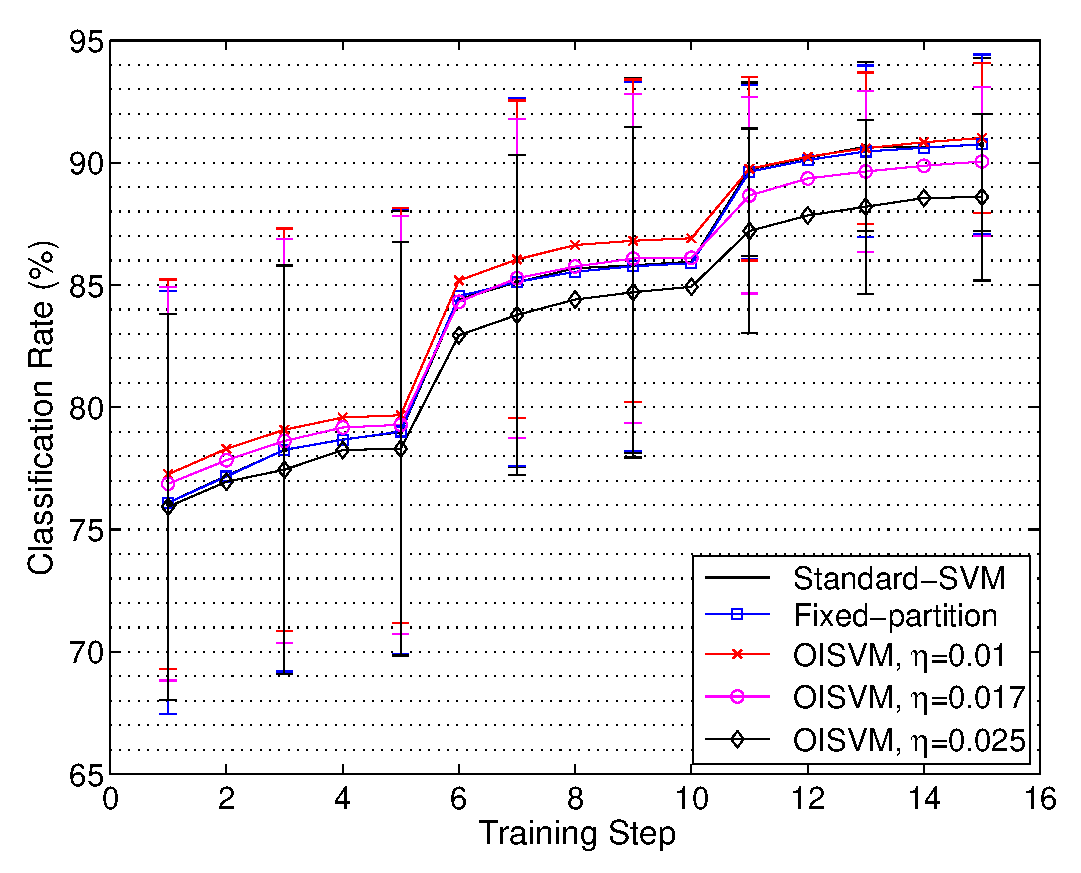
\includegraphics[width=0.47\linewidth]{figs/results/chi_cr} &
  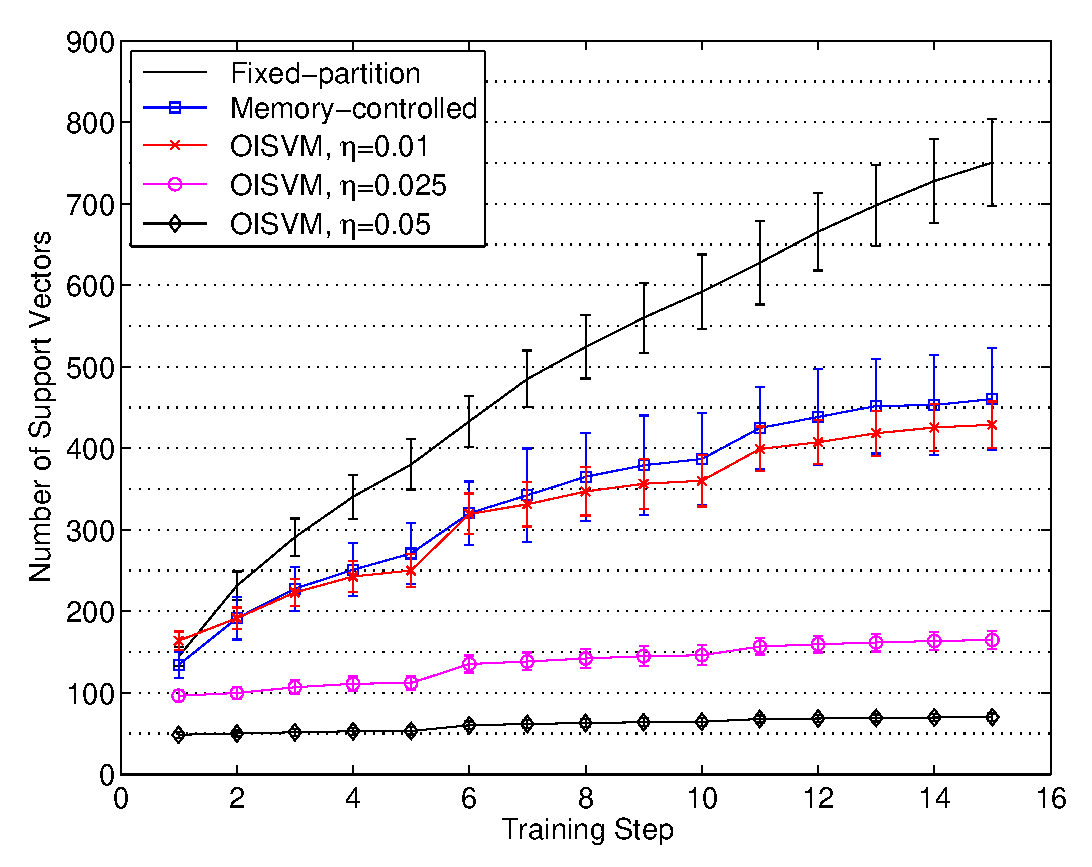
\includegraphics[width=0.47\linewidth]{figs/results/chi_sv} \vspace{0.1cm}\\
  \multicolumn{2}{c}{(a)~Number of support vectors and classification rate obtained at each incremental step using $\chi^2$ kernel.}  \\
  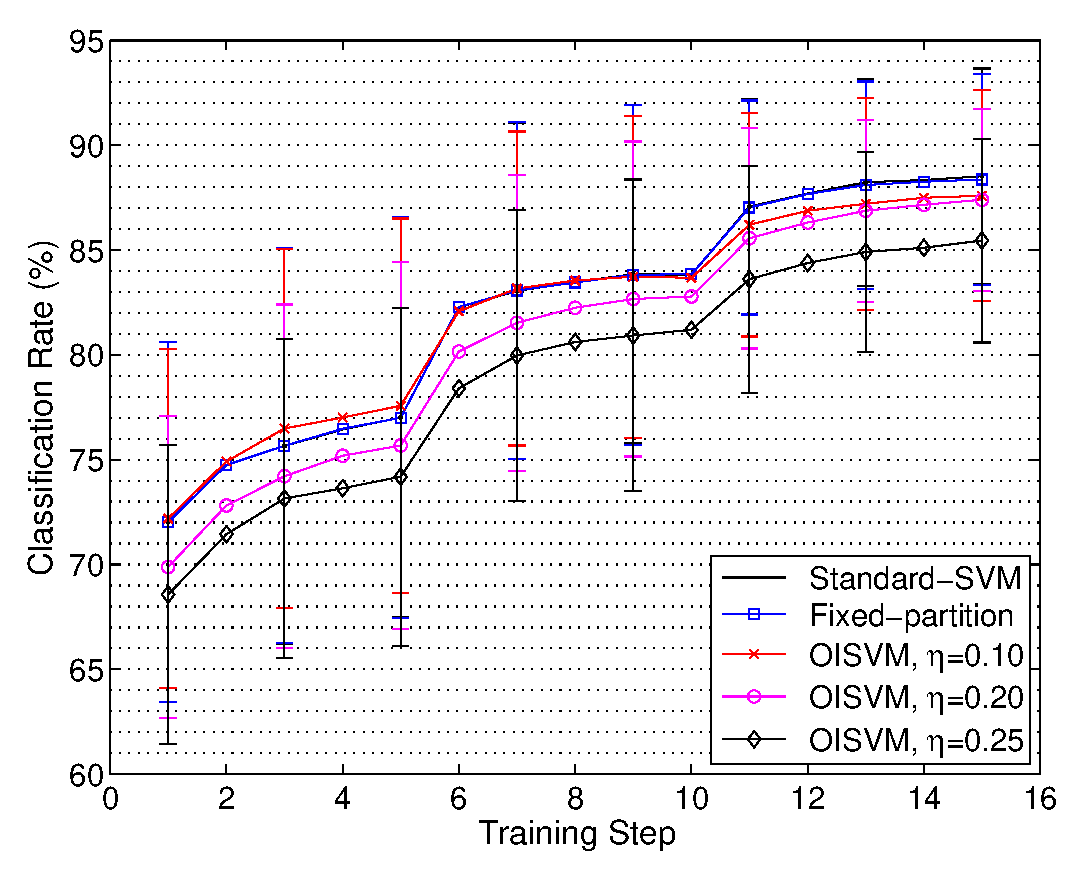
\includegraphics[width=0.47\linewidth]{figs/results/local_cr} &
  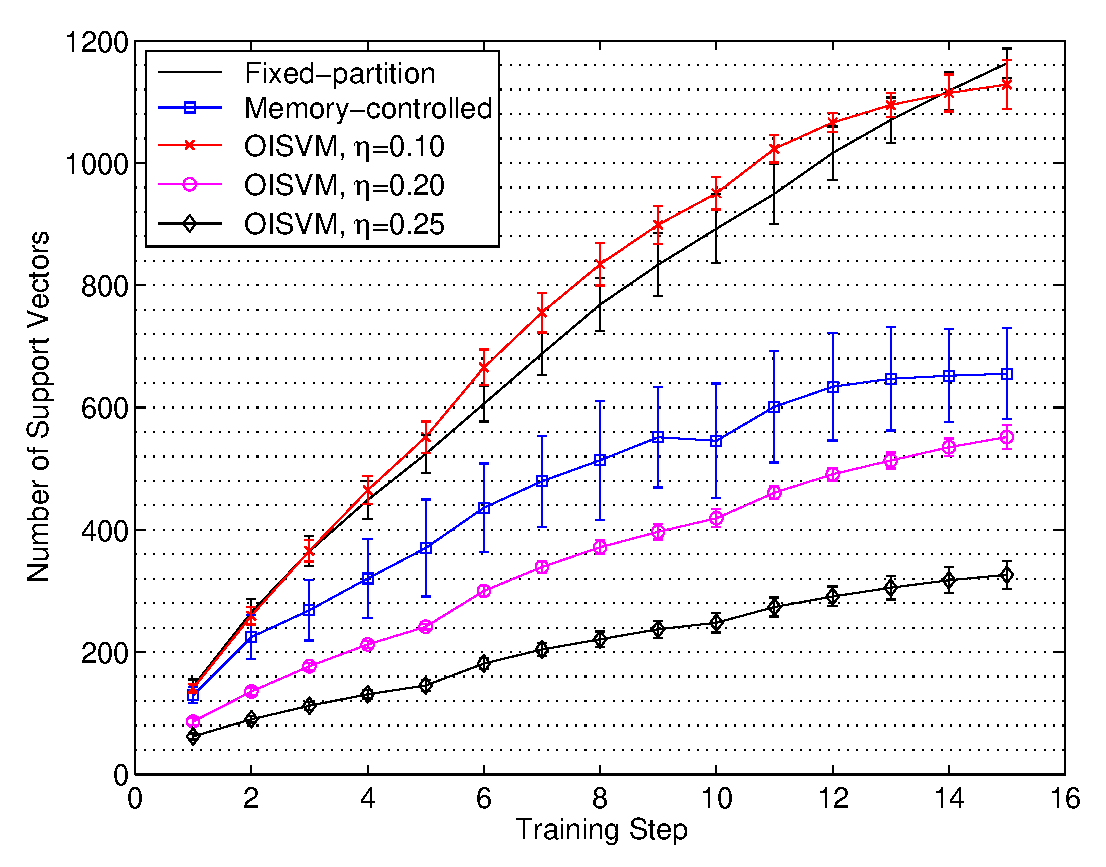
\includegraphics[width=0.47\linewidth]{figs/results/local_sv} \vspace{0.1cm}\\
  \multicolumn{2}{c}{(b)~Number of support vectors and classification rate obtained at each incremental step using local kernel.} \\
  \end{tabular}
\caption{Average results obtained for experiment performed on the IDOL2 database, using
         OISVM with three different values of $\eta$, the fixed-partition and the standard SVM.}
\label{fig:exp:idol}
\end{figure*}


\section{Conclusions}
\label{sec:concl}
We presented a new method to reduce the number of SVs needed by a
Support Vector Machine in an online setting, called OISVMs (Online
Independent Support Vector Machines). OISVMs avoid using in the
solution those support vectors which are linearly dependent of
previous ones in the feature space --- in other words, the kernel
matrix is always kept at full rank. The optimization problem is solved
via an incremental algorithm which benefits of the small size of the
kernel matrix.

We tested the method both on a standard set of benchmark databases and
a real-world case study, namely place recognition in an indoor
environment, from sequences acquired by robot platforms under
different weather conditions and across a time span of several months.

The experimental results show that $(i)$ in the case of
finite-dimensional kernels, OISVMs attain the theoretical limit of
linearly independent support vectors allowed by the feature space,
without losing any accuracy with respect to ordinary SVMs; $(ii)$ in
the case of infinite-dimensional kernels, they dramatically reduce the
number of support vectors at the price of a negligible degradation in
the accuracy. In fact, OISVMs obtain an accuracy up to $0.063\%$ worse
than SVMs with less than $5\%$ of the support vectors of a standard
SVM on a set of standard benchmark databases; whereas, on the
real-world application, we get as few as one third of the SVs required
by the fixed-partition method, while retaining essentially the same
accuracy.

A current limitation of the algorithm is that it requires to store in
memory all training data. This is unfeasible for applications like
place recognition by robot platforms, as it might lead to a memory
explosion. A possible solution might be to combine the OISVM with the
KNN-SVM algorithm \cite{zhang:cvpr06}, so to keep separated the data
storage from the discriminative classification. Another possibility is
to discard training data in a principled way, so to minimize the
effect on the SV solution. Future work will focus on this issue.


\section*{Acknowledgment}
The authors would like to thank...

% ------------------------------------------------------------------------ 

{\small
\bibliographystyle{IEEEtran}
\bibliography{paper}
}

% ------------------------------------------------------------------------ 

\begin{biography}{Francesco Orabona}
Biography text here.
\end{biography}

\begin{biography}{Claudio Castellini}
Biography text here.
\end{biography}

\begin{biography}{Barbara Caputo}
Biography text here.
\end{biography}

\begin{biography}{Jie Luo}
Biography text here.
\end{biography}

\begin{biography}{Giulio Sandini}
Biography text here.
\end{biography}

\end{document}
